\begin{figure}[t]
  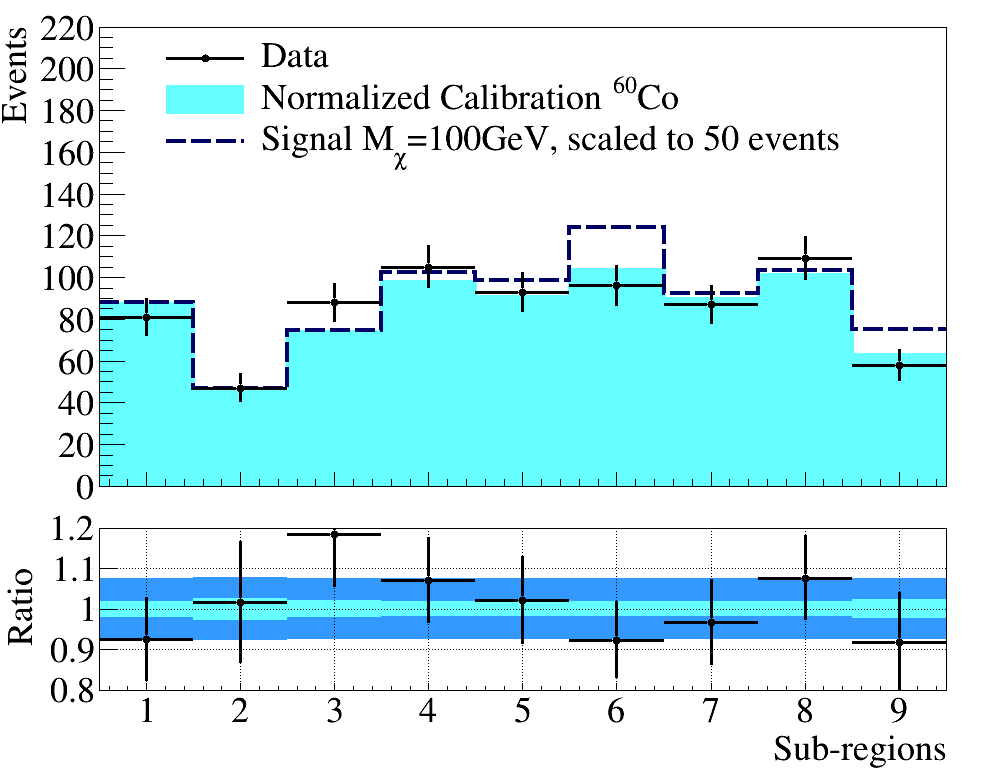
\includegraphics[width=\linewidth]{data_vs_bkg.png}
  \caption{Distribution of  observed events  in the region of interest (data points), along with the normalized distribution from calibration data (filled histogram). The bottom panel displays the ratio
between data and expected background, where the light  and dark blue shaded areas represent the statistical and systematic uncertainty 
on the background expectation, respectively. The expected signal for a WIMP mass of 100\,GeV/c$^2$ (blue dashed), normalized to a total of 50 events, is also shown.}
  \label{fig:dataVSbkg}
\end{figure}


\section{Results and Discussion}
\label{sec:results}

This search is performed using XENON100 Run-II science data, which corresponds to an exposure of 34\,$\times$\,224.6\,kg\,$\cdot$\,days. 
A total of 764 events are observed in the region of interest and no evidence of dark matter can be assessed based on an expected background of
$756 \, \pm \, 5 \,{\rm (stat)} \, \pm 55\, {\rm (syst)}$ events. 
Figure~\ref{fig:dataVSbkg} shows the distribution of  events  in the region of interest, where the bottom panel displays the ratio
between data and expected background. The light and dark blue shaded areas represent the statistical and systematic uncertainty 
on the background expectation, respectively. The expected signal for a WIMP mass of 100\,GeV/c$^2$, normalized to a total of 50 events, is also shown.



\begin{figure}[t]
  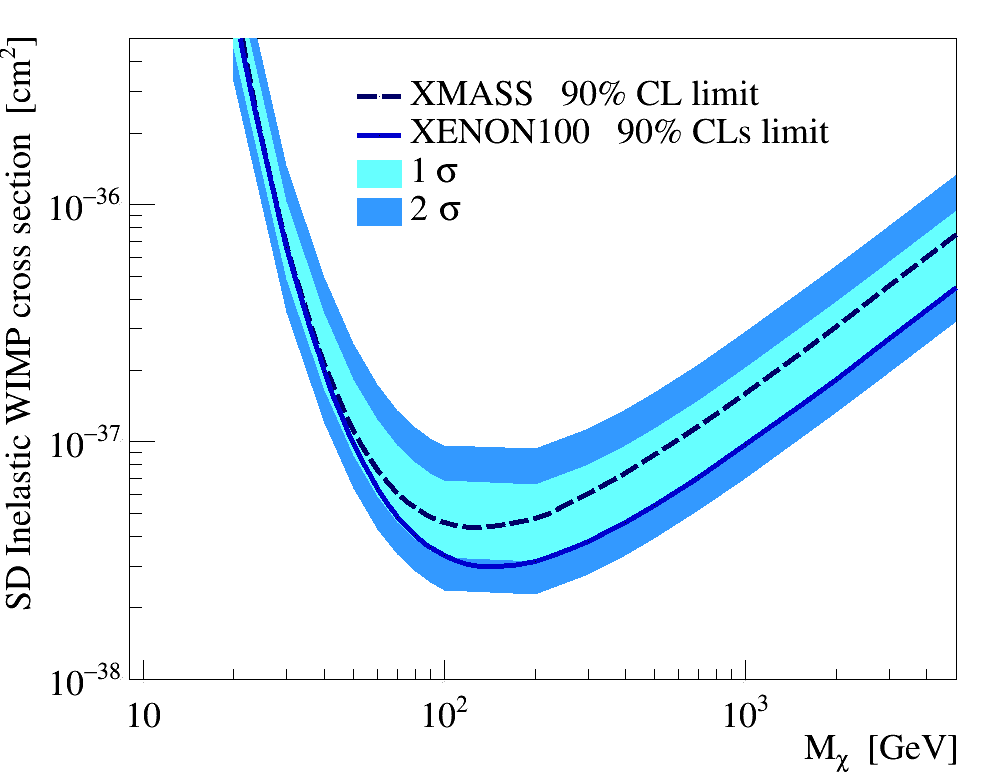
\includegraphics[width=\linewidth]{limit_reb.png}
  \caption{Upper limit (blue curve) on the spin-dependent, inelastic WIMP-nucleon cross section as a function of WIMP mass.  
	  %The expected median sensitivity (dashed curve) along with 
	  The expected one (light shaded area) and two (dark shaded area) standard deviation uncertainty is also shown. 
	  This result is compared to the upper limit (at 90\% C.L.) obtained by the XMASS experiment (dashed line)~\cite{Uchida:2014cnn}.}
  \label{fig:limits}
\end{figure}

This result is interpreted via a binned profiled likelihood approach by means of the test statistic $\tilde{q}$
and its asymptotic distributions, as  described in \cite{asympt}. 
Assuming  an isothermal WIMP halo with a local density of $\rho_{\chi} \, = \, 0.3$\,GeV/cm$^3$, a local circular velocity of $v_0 \,= \, 220$\,km/s, 
a galactic escape velocity of $v_{\rm{esc}} \, = \, 544$\,km/s~\cite{Smith:2006ym}  
and the nuclear structure factors as computed in~\cite{Baudis:2013bba}, 
a 90\% CL$_s$~\cite{cls} confidence level upper limit is set on the spin-dependent inelastic WIMP-nucleon cross section as a function of the WIMP mass. 
%\sout{We employ the nuclear structure factors as calculated in \cite{Baudis:2013qla}, based on state-of-the-art large-scale shell-model calculations, with chiral effective field theory WIMP-nucleon currents.}



Our result is shown in Figure~\ref{fig:limits}, together with its expected one and two sigma statistical variation.
The most constraining limit is  set for a WIMP of mass 100\,GeV/c$^2$ to a cross section of $3.3 \times 10^{-38}$\,cm$^{2}$ (at 90\% CL$_s$ confidence level). 

This result is compared to the one obtained by the XMASS experiment~\cite{Uchida:2014cnn}, a single phase liquid xenon detector, which used a fiducial volume containing 41\,kg of LXe and 165.9~live days of data. 


While these upper limits are not competitive to spin-dependent, elastic scattering results, as obtained by XENON100~\cite{Aprile:2013doa} and LUX~\cite{Akerib:2016lao} 
(bounding the cross section to be $<\,1 \times 10^{-40}$\,cm$^{2}$, at 90\% C.L.,  for a 100\,GeV/c$^2$ WIMP), 
%(with a cross section minimum of $\sim2 \times 10^{-40}$\,cm$^{2}$, at 90\% C.L.,  for a 100\,GeV/c$^2$ WIMP), 
our results are the most stringent for the spin-dependent inelastic channel, and set the stage for a sensitive search of inelastic WIMP-nucleus scattering in running or upcoming liquid xenon experiments such as XENON1T~\cite{Aprile:2015uzo}, XENONnT~\cite{Aprile:2015uzo},  LZ~\cite{Akerib:2015cja}, and DARWIN~\cite{Aalbers:2016jon}. In these larger detectors, with lower intrinsic backgrounds from $^{85}$Kr and $^{222}$Rn decays, and improved self-shielding, the electronic recoil background will be reduced by a few orders of magnitude with respect to XENON100, and ultimately limited by solar neutrino interactions~\cite{Baudis:2013qla}. 
The discovery of this interaction channel would be a clear signature for a spin-dependent nature of the dark matter interaction, and would provide a potential handle  to constrain the WIMP mass with data from one experiment only~\cite{Baudis:2013bba,McCabe:2016aof}.

\section*{Acknowledgments}
We gratefully acknowledge support from the National Science Foundation, Swiss National Science Foundation, Deutsche Forschungsgemeinschaft, Max Planck Gesellschaft, German Ministry for Education and Research, Netherlands Organisation for Scientific Research, Weizmann Institute of Science, I-CORE, Initial Training Network Invisibles (Marie Curie Actions, PITNGA-2011-289442), Fundacao para a Ciencia e a Tecnologia, Region des Pays de la Loire, Knut and Alice Wallenberg Foundation, Kavli Foundation, and Istituto Nazionale di Fisica Nucleare. We are grateful to Laboratori Nazionali del Gran Sasso for hosting and supporting the XENON project.
